% Goal: Informal literature review (~5 pages) on the state of valuing urban ecosystem services
% Andie Creel / Started November 2026
%
% Each section opens with Andie's outline bullets (outline.md) and candidate citations as comments.
% Candidate keys come only from Andie's existing .bib files. Keys not from
% Dissertation/references.bib are tagged with their source bib. Copy entries into ../references.bib as they get cited.

\documentclass[12pt]{article}

% Language setting
\usepackage[english]{babel}

% Set page size and margins
\usepackage[letterpaper,top=2cm,bottom=2cm,left=3cm,right=3cm,marginparwidth=1.75cm]{geometry}

% Useful packages
\usepackage{amsmath}
\usepackage{amssymb}
\usepackage{graphicx}
\usepackage{tikz}
\usetikzlibrary{arrows.meta, decorations.pathreplacing}
\usepackage{array}
\usepackage{booktabs}
\usepackage{caption}
\usepackage{todonotes} % for making comments
\usepackage{natbib}
\usepackage{xurl} % lets long URLs in the bibliography break across lines
\usepackage[colorlinks=true, allcolors=blue]{hyperref}

% Usage: \rev{Author}{comment text}
\newcommand{\rev}[2]{\todo[inline, size=\small, color=yellow!40]{\textbf{#1:} #2}}


\title{The State of Valuing Urban Ecosystem Services -- An Informal Review }
\author{Andie M. Creel}
\date{\today}

\begin{document}
\maketitle

% ------------------------------------------------------------------------------
\section{Conceptualizing, Characterizing, and Measuring Urban Ecosystem Services}\label{sec:intro}
% ------------------------------------------------------------------------------

There is an extensive literature on the services that urban natural assets, such as parks, street trees, coastlines, wetlands, and small lakes and rivers, provide to people. Urban nature can provide heat control, improve air and water quality, mitigate flooding, offer a place to recreate, enhance physical and mental health, and promote social and cultural well-being \citep{keelerSocialecologicalTechnologicalFactors2019, baro_mapping_2016}. The number of studies quantifying these services has been rising for two decades, and this trend accelerated after 2015 \citep{maReviewMethodsQuantifying2025}. Two recent reviews each cover more than 850 publications \citep{veerkampReviewStudiesAssessing2021, maReviewMethodsQuantifying2025}. Cooling and recreation get the most attention. Local temperature regulation accounts for 36 percent of the studies, and recreation and aesthetic appreciation account for another 23 percent \citep{veerkampReviewStudiesAssessing2021}. Large, publicly owned natural assets, such as parks, are studied most often \citep{veerkampReviewStudiesAssessing2021, maReviewMethodsQuantifying2025}.

Despite the size and scope of the existing literature, there is no shared definition of ``urban ecosystem service,'' and that ambiguity hinders researchers' ability to translate results into feasible actions \citep{tanConceptualFrameworkUntangle2020}. Half of the more than 300 papers they review do not define what an ecosystem service is \citep{tanConceptualFrameworkUntangle2020}. The ambiguity and variety of definitions may be due in part to the interdisciplinary nature of the topic, but definitions also vary within fields \citep{boydWhatAreEcosystem2007}.  In addition to the variety in `what' is being measured, the methods used to measure ecosystem services vary tremendously \citep{veerkampReviewStudiesAssessing2021}, with \citet{maReviewMethodsQuantifying2025} identifying at least 47 methods for quantifying urban ecosystem services.

Flooding shows how far the words move. \citet{haines-youngLinksBiodiversityEcosystem2010} lay out a ``cascade'': it starts with an ecological structure, which then provides some sort of function, and that function presumably serves and benefits people. Many urban studies follow this `cascade' framework \citep{baro_mapping_2016, veerkampReviewStudiesAssessing2021}. In \citeauthor{haines-youngLinksBiodiversityEcosystem2010}'s \citeyearpar{haines-youngLinksBiodiversityEcosystem2010} example, a wetland is the ecosystem and it functions to slow surface water. Because flood control is beneficial to people, the wetland's function counts as an ecosystem service. In contrast, \citet{gomez-baggethunClassifyingValuingEcosystem2013} call the percolation of rain through soil and vegetation a function, and make the distinction that the flood control is the ecosystem service. \citet{boydWhatAreEcosystem2007} call the wetland itself the service, the flood control a benefit, and the ecosystem's functions as inputs to services rather than services themselves. Even as the author of this paragraph, I get confused just writing it! The point is that across these three papers, preventing floods is a service in one, and a benefit in another, and a wetland is a structure in one and the service itself in another.\footnote{According to Google Scholar, \citet{haines-youngLinksBiodiversityEcosystem2010} are cited 2,732 times, \citet{gomez-baggethunClassifyingValuingEcosystem2013} are cited 2,797 times, and \citet{boydWhatAreEcosystem2007} are cited 4,175 times. So, it's not as if any of these definitions are fringe!}    

Additionally, the literature rarely measures the benefits of ecosystem services to people. This is another major hindrance to researchers' ability to influence decision-makers. Fifty-nine percent of reviewed papers quantify ecosystem properties, but a minority of current literature explicitly states the benefits of urban ecosystem services to people \citep{veerkampReviewStudiesAssessing2021}. Even fewer papers measure benefits in monetary units, such as dollars. By not measuring the value of ecosystem services to people, researchers limit their ability to inform policy-makers, non-profits, businesses, and corporations about how to make informed decisions regarding urban natural assets. Research on urban nature-based solutions to climate change has underexamined their socioeconomic dimensions, and there is little city-scale empirical evidence on the economic benefits \citep{mcphearsonGlobalSynthesisRegional2025,herisPilotingUrbanEcosystem2021}. The value of urban ecosystem services remains far more uncertain than what the services themselves are \citep{keelerSocialecologicalTechnologicalFactors2019}.

Not understanding how ecosystem services benefit people is consequential for investing in new urban natural assets (\textit{e.g.,} planting street trees), restoring degraded ones (\textit{e.g.,} wetlands), and conserving current natural assets from development pressure. Without a dollar value on the benefit these natural assets provide, a city cannot run a benefit-cost analysis of planting street trees or restoring a stream, whether that analysis is to justify its own budget or to compete for grant money. It is also hard to know if businesses or corporations may have a private incentive to pay for the establishment or restoration of urban natural assets. Arguing that a city with a limited budget should allocate some of that budget to increasing ecosystem services requires knowing how the benefits of those services compare with other obligations of the city, such as schools, roads, and safety measures. Arguing that a business or corporation should invest in natural assets requires establishing how the ecosystem services from those assets will increase its profits, either through revenue gains or cost savings. Non-profits, such as land trusts and park conservancies, also restore and maintain urban natural assets. They do not need to make a profit, but they benefit when they can tell funders and city partners what a dollar spent on natural assets returns in terms of benefits to people.  

The rest of this review proceeds as follows. First, I define natural assets, ecosystem functions, and benefits, and briefly address cultural and spiritual services (Section~\ref{sec:define}). Second, I summarize the well-established functions of urban green space, trees, and water, along with the dollar value of the benefits when available (Section~\ref{sec:established}). Third, I describe how unequally natural assets are distributed across urban neighborhoods (Section~\ref{sec:distribution}). Fourth, I point to a remaining gap in measuring the beneficial functions of urban animals (Section~\ref{sec:animals}). Finally, I turn from measuring the functions of existing natural assets to asking who builds new ones and how research can inform that investment (Section~\ref{sec:building}).

% ------------------------------------------------------------------------------
\section{What Is an Ecosystem Service?}\label{sec:define}
% ------------------------------------------------------------------------------
The literature's inability to agree on a definition of ``ecosystem service'' limits its ability to build consensus on established results and on what remains to be understood. So, like so many before me, I will try to define three key terms related to ecosystem services so we can communicate with each other! 

First, I define a natural asset as a stock of nature measured in its own units, such as acres of park, area of tree canopy, number of foxes, miles of trail, or surface area of a lake. A park, for example, is not an ecosystem service. It is a natural asset. The second is the ecosystem function that a natural asset provides, which I define as a function of a natural asset. A single natural asset may provide many functions. For example, a city park can function in many ways; it can create a cooler microclimate, a place to recreate, and control stormwater. The third key term is the function's benefit to people, which I define as the value of an ecosystem function to people. This benefit should, ideally, be measured in dollars so that it is easy to compare the benefits provided by natural assets (through their functions) with other benefits. 

Figure~\ref{fig:cascade} shows the three together. It is often possible to measure that a service is being provided without knowing its benefit. Consider a municipal government. It may know that trees (a natural asset) provide cooling (a function), but without some measure of the benefit of that cooling, it is hard to decide whether to spend the municipal budget on planting trees or on other beneficial services like roads or safety. Decision-makers who determine whether a city will have more or fewer natural assets therefore need a measure of the benefits of ecosystem services, so that managers can weigh those benefits against the other outcomes they are managing for.

% --------
% Figure 1
% --------

\begin{figure}[t]
\centering
\caption{Three Key Terms Regarding Ecosystem Services}
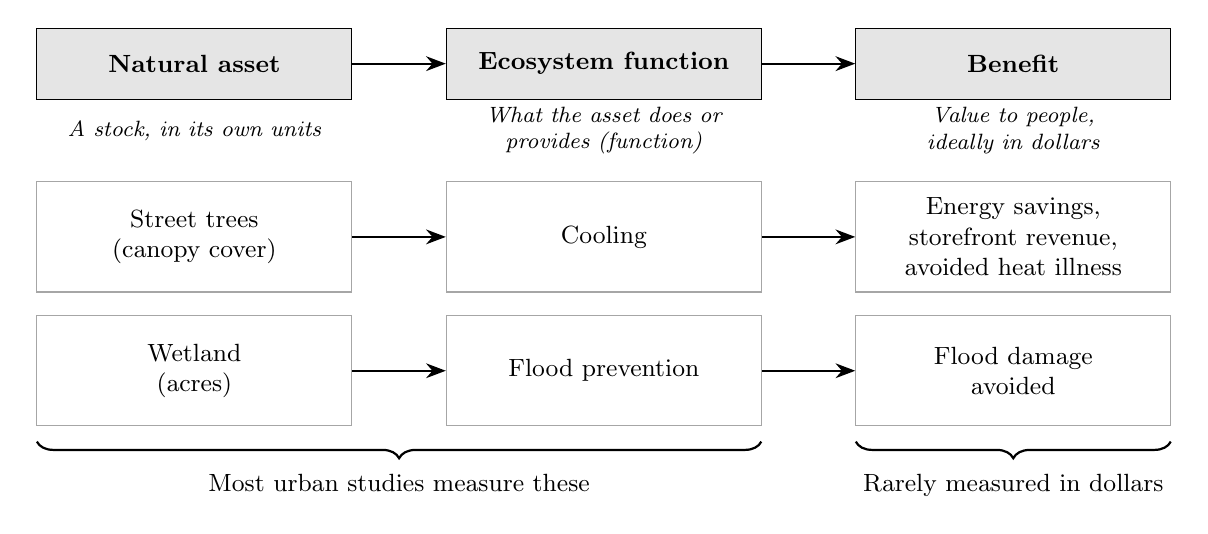
\begin{tikzpicture}[
  font=\small,
  head/.style={draw, fill=gray!20, minimum width=4cm, minimum height=0.9cm, align=center, font=\small\bfseries},
  def/.style={text width=4cm, align=center, font=\footnotesize\itshape},
  ex/.style={draw=gray!70, minimum width=4cm, minimum height=1.4cm, align=center},
  arr/.style={-{Stealth[length=2.5mm]}, thick}
]
  % Column headers and definitions
  \node[head] (a) at (0,0)    {Natural asset};
  \node[head] (s) at (5.2,0)  {Ecosystem function};
  \node[head] (b) at (10.4,0) {Benefit};
  \draw[arr] (a) -- (s);
  \draw[arr] (s) -- (b);
  \node[def] at (0,-0.85)    {A stock, in its own units};
  \node[def] at (5.2,-0.85)  {What the asset does or provides (function)};
  \node[def] at (10.4,-0.85) {Value to people, ideally in dollars};
  % Example: trees
  \node[ex] (a1) at (0,-2.2)    {Street trees\\(canopy cover)};
  \node[ex] (s1) at (5.2,-2.2)  {Cooling};
  \node[ex] (b1) at (10.4,-2.2) {Energy savings,\\storefront revenue,\\avoided heat illness};
  \draw[arr] (a1) -- (s1);
  \draw[arr] (s1) -- (b1);
  % Example: wetland
  \node[ex] (a2) at (0,-3.9)    {Wetland\\(acres)};
  \node[ex] (s2) at (5.2,-3.9)  {Flood prevention};
  \node[ex] (b2) at (10.4,-3.9) {Flood damage\\avoided};
  \draw[arr] (a2) -- (s2);
  \draw[arr] (s2) -- (b2);
  % Where the literature is
  \draw[decorate, decoration={brace, mirror, amplitude=6pt}, thick]
    (-2,-4.8) -- (7.2,-4.8) node[midway, below=8pt] {Most urban studies measure these};
  \draw[decorate, decoration={brace, mirror, amplitude=6pt}, thick]
    (8.4,-4.8) -- (12.4,-4.8) node[midway, below=8pt] {Rarely measured in dollars};
\end{tikzpicture}
\label{fig:cascade}

\vspace{0.5em}
\begin{minipage}[t]{0.8\linewidth}
\footnotesize \noindent Natural assets, ecosystem functions, and benefits as defined in this review. Most papers measure the asset and the function it provides \citep{veerkampReviewStudiesAssessing2021}. Far fewer measure the benefit in dollars. This is only an illustrative diagram, and is not meant to be a census of the functions and benefits of street trees or wetlands!
\end{minipage}
\end{figure}

Natural capital accounting puts heavy emphasis on a technical procedure for expressing monetary benefit in units of the natural asset \citep{fenichelMeasuringValueGroundwater2016, fenichelNewEra2024}. In this framework, one acre of park, one tree, or one mile of trail has a dollar value, in the same way that produced capital has a price. \citet{fenichelNaturalCapitalMetaphor2014}, for example, recover an accounting price for a pound of Gulf of Mexico reef fish. Eventually, having every natural asset priced this neatly would be amazing; natural capital accounting could be considered the gold standard for valuing a natural asset's benefits. However, it is technically very hard to connect a unit of benefit back to a unit of the asset. Doing so requires understanding the feedback loops between the natural asset, the human behavior that affects it, and the institutions that shape that behavior \citep{fenichelNewEra2024}. Therefore, \textit{measuring the benefit of urban natural assets perfectly should not be the enemy of measuring the benefit of these assets and their functions at all!} 

A brief caveat: Cultural and spiritual ecosystem services fit less neatly into this framework. It is not always clear what the natural asset is, what function it provides, or how to put a dollar value on the benefit. A community may value a river for its spiritual significance, which is tied directly to the river, not to a service that flows from it. Species valued for their mere existence are less often valued formally because their non-market values are hard to derive \citep{maher_economics_2020}, and \citet{boydWhatAreEcosystem2007} make a similar point about the emotional benefits of contact with nature. Culturally important species, which frequently matter to Indigenous Peoples and ethnic groups, are also more likely than other species to lack basic biological data \citep{reyes-garcia_biocultural_2023}. \citet{diepEmpoweringCitiesGlobally2025} argue that the need to make a ``business case'' for nature-based solutions has given priority to economic valuation and undermined Indigenous Peoples' worldviews and other ways of relating to nature. However, I do not think that this should prevent us from valuing other ecosystem services in dollars. In my opinion, a dollar value is not meant to replace those other ways of valuing nature. It is instead meant to keep nature in the equation when a city weighs planting trees against schools and roads (\textit{i.e.,} it is a useful unit, but not a more important one). I do not try to settle whether or how cultural and spiritual services should be valued in dollars. The rest of this review focuses on services whose assets, functions, and benefits are easier to define.



% ------------------------------------------------------------------------------
% ------------------------------------------------------------------------------
% OUTLINE:
% * What's established -- cooling, stormwater, recreation, health (physical and mental health)
%     * Established lit focuses mostly on value of green space / water / not impervious surfaces
%         * Tbh this stuff doesn't really need new research on it the service exists -- it's clear from
%           lit that these services exist
%         * What is needed is who benefits from these
%     * A big gap in ecosystem services provided by bugs and animals in urban settings (subsection below)


% ------------------------------------------------------------------------------
\section{Established Functions of Urban Natural Assets}\label{sec:established}
% ------------------------------------------------------------------------------


There are well-established ecosystem functions provided by urban green space, street trees, waterways, and wetlands (natural assets). These functions include urban heat mitigation, stormwater management, air purification, recreation, and health benefits (both physical and mental). \cite{keelerSocialecologicalTechnologicalFactors2019} provide a summary table of urban natural assets and the ecosystem functions they provide that I find particularly useful for orienting to which asset does what function. I include their Table 1 as Figure \ref{fig:keeler} in this review. 

% --------
% Figure 2
% --------
\begin{figure}[t]
\centering
\caption{Taken from Table 1 of \citet{keelerSocialecologicalTechnologicalFactors2019}.} 
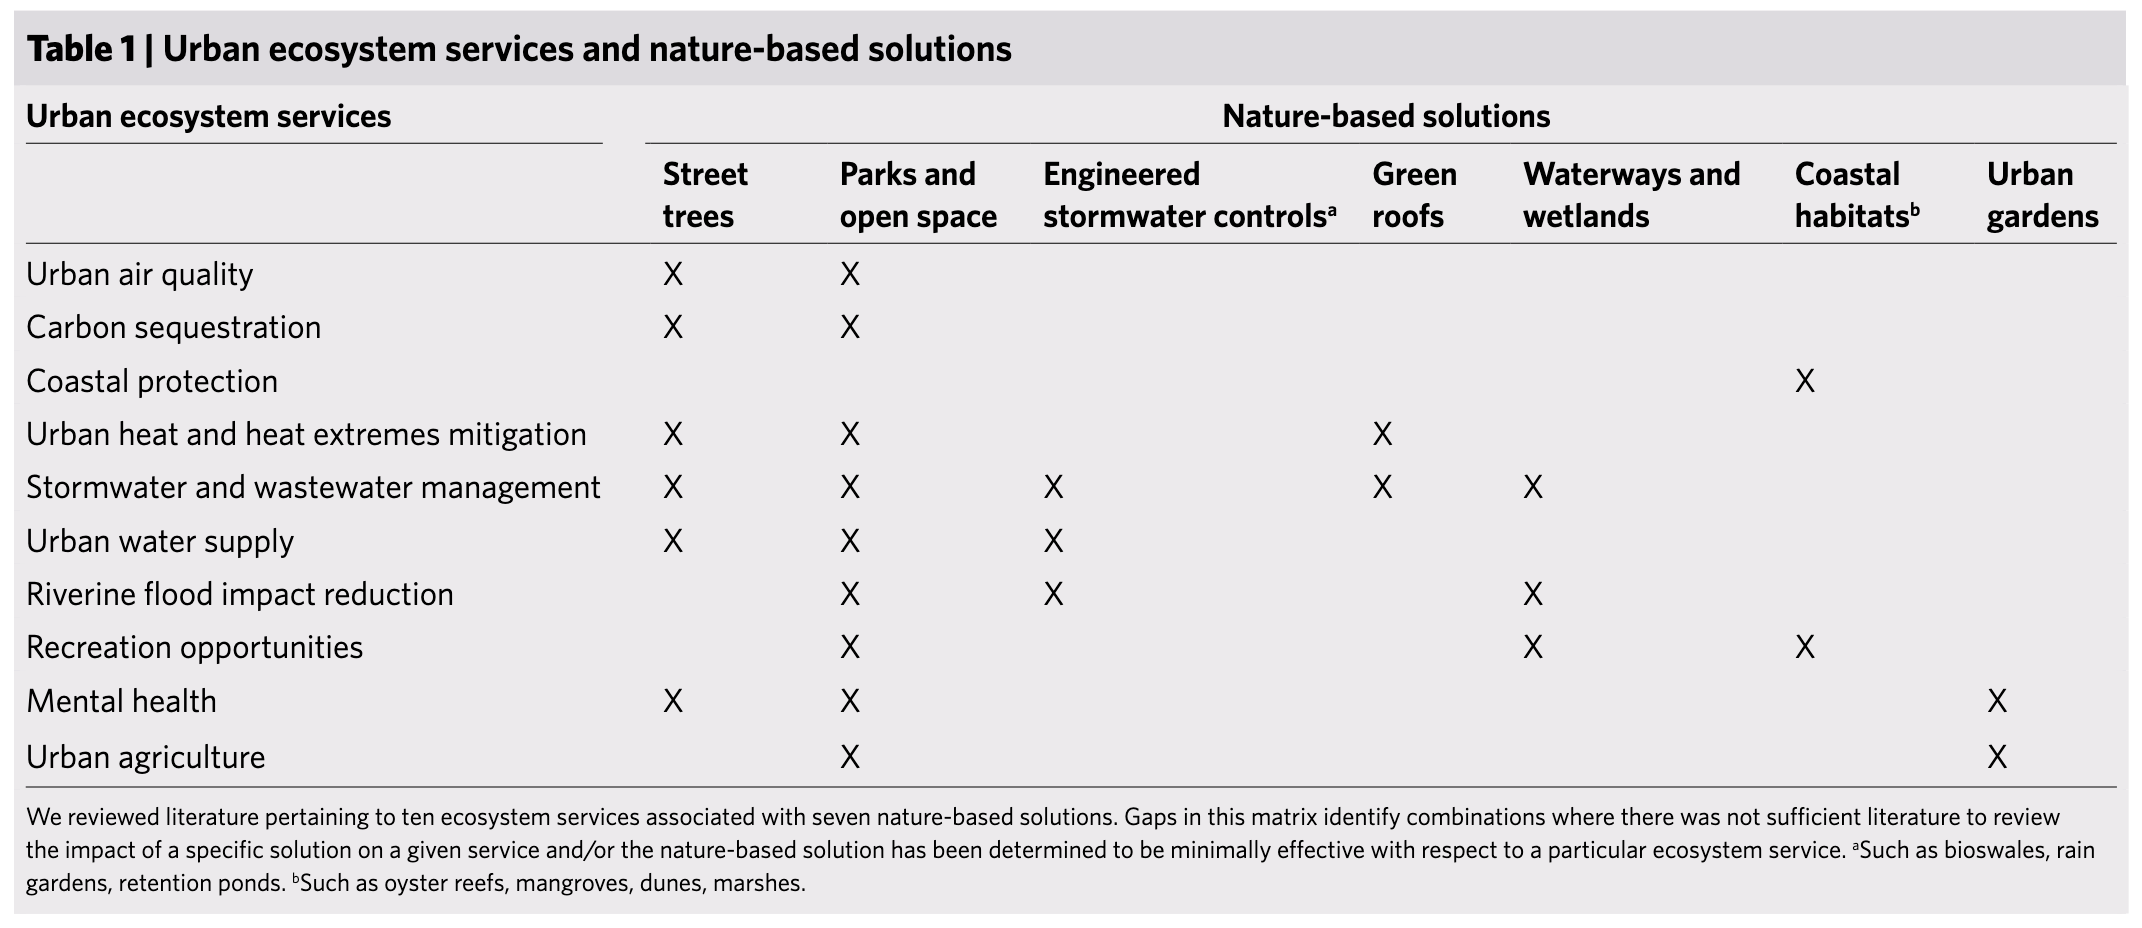
\includegraphics[width=\textwidth]{../figures/Keeler_table_1.png}
\label{fig:keeler}
\vspace{0.5em}
\begin{minipage}[t]{0.8\linewidth}
\footnotesize \noindent What \cite{keelerSocialecologicalTechnologicalFactors2019} call nature-based solutions, I call natural assets. What they call urban ecosystem services, I refer to as ecosystem functions.
\end{minipage}
\end{figure}

Literature reviews also agree on which natural assets get the most attention. Green space of an unspecified type (30 percent) and parks and other natural green areas (26 percent) together make up more than half of the papers that \citet{veerkampReviewStudiesAssessing2021} review. Abandoned land makes up only 2 percent, but may be the best opportunity for the establishment of new natural assets. \citet{maReviewMethodsQuantifying2025} find a similar ordering. Woodlands, parks, and water bodies are studied more often than rain gardens, private gardens, and allotments, and green roofs and green walls are studied least. 

The functions that are best understood are regulating functions. Microclimate, water, and gas regulation are the most frequently quantified \citep{maReviewMethodsQuantifying2025}, and most studies measure them as physical changes, such as lower air temperatures, reduced stormwater runoff, or pollutants removed from the air and water \citep{veerkampReviewStudiesAssessing2021}.

The benefits of these functions are much less understood. Only 3 percent of studies rely solely on what \citet{veerkampReviewStudiesAssessing2021} call service indicators, which measure whether a natural asset meets people's demand for the function it provides. When studies do estimate a dollar value, simple methods dominate \citep{maReviewMethodsQuantifying2025}. Value transfer, which borrows values from earlier studies, accounts for about 47 percent of monetary valuations, and cost-based approaches, such as damage costs avoided or replacement costs, account for another 36 percent \citep{maReviewMethodsQuantifying2025}. Estimates also vary widely. Past studies report annual net benefits of \$5 to \$402 per urban tree, a range that suggests high uncertainty in the methods used to value trees, the returns to urban nature across cities, and which functions of a natural asset are included in a valuation study \citep{keelerSocialecologicalTechnologicalFactors2019}. Of the ten services that \citet{keelerSocialecologicalTechnologicalFactors2019} review, mental health has the most uncertain value, even though there is strong evidence that engaging with nature and living near urban green space improves public health \citep{mcphearsonGlobalSynthesisRegional2025}. Finally, the value of urban nature is rarely compared with the built alternatives a city could pay for instead, such as air conditioning, seawalls, or levees \citep{keelerSocialecologicalTechnologicalFactors2019}.
% Checked against full text (Zotero; Ma and Yang via PDF): Veerkamp et al. (GBI types: unspecified 30%, parks and (semi-)natural
% green areas 26%, grey-connected 17%, water 10%, building greens 8%, gardens 6%, abandoned land 2%; ecosystem indicators 59%;
% service indicators alone 3% [another ~10% combine ecosystem + service indicators]; service indicator example = thermal comfort).
% Ma and Yang (woodlands, parks, water bodies > rain gardens, private gardens, allotments; green walls/roofs least; microclimate,
% water, gas regulation most studied; "simple methods dominated the monetary value assessment"; value transfer 46.82% and cost
% approaches 35.53% "of studies" estimating monetary values; cost approaches incl. damage cost avoided, replacement cost).
% Keeler et al. ($5--$402 per tree; Table 2: mental health is the only service rated "high uncertainty"; value "rarely compared
% with alternative interventions"; Table 2 substitutes incl. home air conditioning, seawalls, levees).
% McPhearson et al. ("strong evidence on the positive public health outcomes from engaging with nature and biodiversity and
% from living near urban green spaces").
% Keeler Table 2 uncertainty ratings, if useful: carbon low; air quality, water supply, recreation low-moderate; heat, stormwater,
% coastal, riverine flood, urban agriculture moderate; mental health high.

% CANDIDATE CITATIONS:
%   Cooling: wongGreeneryMitigationAdaptation2021, mohajeraniUrbanHeatIsland2017,
%            jenerette_ecosystem_2011 [YIBS bib], JMP
%   Cooling -> energy: hanCoolCitiesValue2024, herisPilotingUrbanEcosystem2021
%   Capitalization into housing: klaiberItLessHot2017, netusilEstimatingDemandTree2010, sanderValueUrbanTree2010,
%            albouy_unlocking_2020 [LWCF / prospectus bib]
%   Recreation: creelNationalValueLocal2026, dayValueGreenspace2020, salazarmirandaDesirableStreetsUsing2021,
%            kazmierczakContributionLocalParks2013, tplCityParkFacts2025,
%            hamstead_geolocated_2018, donahue_using_2018, venter_urban_2020 [prospectus recreation demand bib]
%   Stormwater: none in your bibs -- Andie will supply
%   Health (physical, mental): none on green space in your bibs -- Andie will supply
%            (temperature and health: janzenTemperatureMentalHealth2025, carletonValuingGlobalMortality2022)
%   Who benefits: druppEconomicsInequalityEnvironment2025, fenichelNaturalCapitalEquity2019

The following subsections elaborate on what we know about the functions of urban natural assets and the benefits they provide to cities and their residents.

\subsection{Urban Heat Mitigation}\label{sec:heat}

The natural assets that regulate urban microclimates include trees and other vegetation, such as parks, green roofs, and green walls. A function these assets provide is cooling. Vegetation cools its surroundings through shade and evapotranspiration, which counteracts the urban heat island that makes cities hotter than the surrounding countryside \citep{mohajeraniUrbanHeatIsland2017, wongGreeneryMitigationAdaptation2021}. Greenery on the ground typically lowers peak surface temperatures by 2--9 °C \citep{wongGreeneryMitigationAdaptation2021}, and in Phoenix, vegetation cools the surface by nearly 25 °C relative to bare soil on low-humidity summer days \citep{jenerette_ecosystem_2011}. 

The benefit of cooling has been measured in dollars in several ways. Households in Phoenix have a marginal willingness to pay of \$72 per month for a 1 °F reduction in outdoor temperature \citep{klaiberItLessHot2017}. Urban trees in major U.S.\ cities save energy for indoor cooling worth \$539 million in 2016 \citep{herisPilotingUrbanEcosystem2021}. In my own work, I find that an increase in green space surrounding a business directly increases its revenue by half a percentage point on days at or above 100 °F \citep{creelValueNatureBasedAdaptation2026}.

Many more studies value trees through property prices \citep{sanderValueUrbanTree2010, netusilEstimatingDemandTree2010}, but property prices capture a bundle of services that includes aesthetic beauty, as well. In Toronto, trees cool neighborhoods and save energy, but their total amenity value exceeds the value of these two services \citep{hanCoolCitiesValue2024}. That study also measures value in units of the natural asset itself: a single tree adds 0.45 percent to property prices within a postal code.

\subsection{Stormwater Regulation}\label{sec:stormwater}

For stormwater regulation, natural assets include trees and other permeable surfaces, such as parks and vegetated green infrastructure, that replace impervious pavement and roofs. The function is to intercept and absorb rainfall, which reduces the runoff that cities must otherwise manage \citep{veerkampReviewStudiesAssessing2021, herisPilotingUrbanEcosystem2021}. Most of these studies model reductions in runoff or peak flow, often using the Storm Water Management Model (SWMM), and many examine vegetated features integrated into built infrastructure, such as rain gardens, swales, detention ponds, and constructed wetlands \citep{veerkampReviewStudiesAssessing2021}. 

A large majority of research on urban nature-based solutions focuses on water, especially flooding \citep{mcphearsonGlobalSynthesisRegional2025}. Even so, it is still not clear which types of natural assets reduce flooding and where other solutions are needed \citep{diepEmpoweringCitiesGlobally2025}. Trees, for example, intercept rainfall most effectively during small storms, so they may do little to mitigate flooding during extreme events \citep{herisPilotingUrbanEcosystem2021}.

As far as I am aware, there has been limited work valuing this service in dollars. \citet{herisPilotingUrbanEcosystem2021} estimate that urban trees in major U.S.\ cities intercepted about 2.6 billion cubic meters of rainfall in 2016, which they value at \$425 million. That value is an avoided cost. In cities where stormwater and sewage share the same pipes, heavier stormwater flows raise treatment costs at the wastewater treatment plant and cause sewage to overflow into waterways. \citet{herisPilotingUrbanEcosystem2021} price each cubic meter of rainfall that trees intercept over impervious surfaces at the cost of controlling stormwater, about \$2.58 (2019 USD), and they count only cities with these combined sewers, where the treatment plant is the beneficiary. The estimate therefore does not include avoided flood damage to homes and businesses.
% Checked against full text (Zotero): Veerkamp et al. (stormwater 14% of assessments, after temp 36% and recreation 23%; mainly modelling,
% SWMM common; indicators = runoff/peak flow reduction, water retention; 42% in GBI connected to grey, e.g., raingardens, swales,
% detention ponds, constructed wetlands; Table 1 defn "rainfall is intercepted and stored by vegetation and soil").
% McPhearson et al. ("a large majority of NbS research focuses on water-related challenges, especially flooding").
% Diep and McPhearson ("still needs to understand what types of green stormwater infrastructure can be effective in reducing
% flooding impacts and where other solutions will be needed"). Heris et al. (trees most effective in small storms, "may not
% substantially influence flood mitigation during extreme events"; CSO treatment costs and overflows; $0.009/gal = $2.58/m3 in
% 2019 USD from i-Tree stormwater control costs; interception over impervious surfaces only; valued only for WWTPs in CSO cities).
% For Section 6: Toxopeus and Polzin note stormwater tax cuts for green roofs in parts of Germany spur private investment.


\subsection{Air Purification}\label{sec:air}

For air purification, the natural assets are again trees and other urban vegetation. The function is to remove pollutants, such as particulate matter, from the air people breathe, and tree species with larger leaf area or sticky or hairy leaves remove particulates at a higher rate \citep{keelerSocialecologicalTechnologicalFactors2019}. Air quality regulation accounts for 13 percent of urban ecosystem service studies, and these studies most often measure function by tree characteristics or cover rather than by a specific type of green space \citep{veerkampReviewStudiesAssessing2021}. In Lima, Peru, publicly managed urban trees remove about 27 tons of fine particulate matter (PM2.5) and 319 tons of coarser particulate matter (PM10) each year \citep{morenoContributionUrbanTrees2024}. Where new trees are planted also matters. In a neighborhood of Perugia, Italy, converting marginal farmland into an urban forest would increase PM2.5 removal by 237 percent, while adding street trees would yield smaller gains but place trees closer to pollution sources, better aligning the function with where it is needed \citep{menconiOptimizingLocalRegulating2026}.

At the scale of a whole city, however, the effect is small. Trees reduce city-wide air pollution by less than 1 percent to at most 5 percent, and reducing energy use or switching to cleaner energy may address particulate pollution more effectively \citep{keelerSocialecologicalTechnologicalFactors2019}. \citet{keelerSocialecologicalTechnologicalFactors2019} rate the potential value of urban nature for air quality as low and suggest shifting research away from goals such as mitigating air pollution with street trees and toward nature's contributions to recreation, social cohesion, and physical and mental health.

The benefit to people runs largely through health, which links this service to the health subsection below (Section~\ref{sec:health}). As far as I am aware, few studies value this function in dollars. \citet{liuLinkingUrbanAir2020} come closest. In a choice experiment in Beijing, households would pay \$2.04 per month (2017 USD) for one additional neighborhood park at the sample's average pollution level, but only \$0.59 per month at the lowest pollution level. Willingness to pay for a new neighborhood park increases with residents' exposure to air pollution, whereas pollution has no significant effect on willingness to pay for a new city or national park. The authors interpret this as evidence that neighborhood parks directly purify the air for the communities around them \citep{liuLinkingUrbanAir2020}. The willingness to pay is for the whole park, so it bundles air purification with recreation and everything else a park provides.
% Checked against full text (Zotero): Keeler et al. ("larger leaf area and sticky or hairy leaves increase the removal rate of
% particulate air pollution"; city-scale reductions "minimal, ranging from less than 1% to up to 5%"; cleaner energy / reduced
% energy use "more effectively and permanently" address particulates; Table 2: urban air quality = low potential value;
% "may suggest a shift in emphasis" from mitigating air pollution with street trees toward recreation, social cohesion, health).
% Veerkamp et al. (air quality 13%; "mostly assessed based on characteristics and/or cover of trees", unspecified GBI 42%).
% Moreno et al. (i-Tree; Lima public urban trees remove 26.78 t PM2.5 and 319.22 t PM10 per year).
% Menconi et al. (neighborhood of Perugia; SC4 farmland-to-forest +237.4% PM2.5 removal; street trees SC5 lower gains but
% closeness to pollution sources aligns demand and service delivery).
% Liu et al. (Beijing choice experiment; median WTP CNY 13.77 = USD 2.04 /household/month at sample mean pollution; CNY 3.95 =
% USD 0.59 at sample minimum; CNY 6.75 = USD 1 in 2017; no significant pollution effect for city or national park).
% Left out: "an extra CNY 22 (USD 3.26)" at the sample maximum -- unclear whether that is a total or an increment over 13.77.

\subsection{Recreation}\label{sec:recreation}

For recreation, the natural assets are parks, trails, water bodies, and the tree-lined streets and sidewalks people walk along. The function is to provide a place to recreate and spend leisure time outside. Most outdoor recreation in the United States is local and centered on everyday activities, such as walking, playing with kids or pets, and socializing, so much of it likely occurs within cities \citep{creelNationalValueLocal2026}. Which urban parks people use depends on what those parks offer. In the Twin Cities, parks with water features, more amenities, and trails, and parks in denser neighborhoods, get more visits \citep{donahue_using_2018}. In Beijing, large urban parks get the most visits in total, but neighborhood parks get more visits per unit of area \citep{zhang_recreational_2018}. Demand for this function also rises when other leisure options close. Park visits were a critical source of leisure during the COVID-19 pandemic, when other ways to spend leisure time were forced closed \citep{gengImpactsCOVID19Pandemic2021,venter_urban_2020,dayValueGreenspace2020}. 

Recreation in parks is also social, and the societal trust built in city parks is another function of these natural assets that is not well understood at all. Visits to local parks are associated with more social ties among neighbors in inner-city Manchester \citep{kazmierczakContributionLocalParks2013}, and urban parks in the Netherlands are places where ethnic groups mix and informal interactions can build social cohesion \citep{petersSocialInteractionsUrban2010}. 

It is less clear how much of the visitation to parks is driven by the nature in a park rather than by its other features. Across New York City's 2,143 parks, geolocated social media posts, a proxy for visits, are more common in parks near public transit and bike routes and in parks with water bodies, athletic facilities, and impervious surfaces, but less common in parks with more green space \citep{hamstead_geolocated_2018}. \citet{hamstead_geolocated_2018} conclude that the kinds of green space in many parks may not motivate visits. Posts are also less common in parks in neighborhoods with a larger share of minority residents. The authors read this as a sign that parks in those neighborhoods may be less accessible or of lower quality, which I return to in the section on distribution below (Section~\ref{sec:distribution}).

The benefit of this service has been measured in dollars. In a working paper, Eli Fenichel and I use a travel-cost model to estimate the value of local outdoor recreation over seven three-year periods from 2003 to 2023, and find it is consistently between \$5 and \$6 per trip (2023 USD) \citep{creelNationalValueLocal2026}. This value aggregates to about \$93 billion per year nationally in 2021--2023. Park proximity and open space are also capitalized into property values. Reductions in crime ``unlocked'' almost \$7 billion in property value near parks in Chicago, New York, and Philadelphia, while about \$10 billion remains locked in \citep{albouy_unlocking_2020}. Stated preference studies can value the quality of urban green space. Germans would, on average, pay \texteuro 20.25 per month to make the green space closest to them more natural \citep{bronnmannValueNaturalnessUrban2023}. 

Finally, \citet{wuOpenSpaceUS2023} estimate that about 97 percent of U.S.\ metropolitan areas have too little open space in their developed areas, so conserving more open space there would raise social welfare.

% Albouy abstract: ~$7B unlocked in Chicago, NY, Philadelphia; two-fifths of potential park-proximity value, $10B, remains locked in.
% Checked against Zotero abstracts / full text: Donahue et al. (water features, amenities, trails, higher pop. density -> more
% visits); Zhang and Zhou (large urban and cultural relics parks most visits; neighborhood parks highest visits per area);
% Geng et al. (park visitation up since Feb 16, 2020 in most countries, Google mobility data); Venter et al. (+291% vs 3-yr
% average for same days; ~86,000 extra activities/day; pedestrians and cyclists "appeared to intensify activity on trails with
% higher greenviews and tree canopy cover"); Kazmierczak (Greater Manchester; park visits associated with social ties);
% Peters et al. (five Dutch urban parks; ethnic groups mingle, informal interactions stimulate cohesion); Hamstead et al.
% (2,143 NYC parks; Flickr/Twitter; + transit, bike routes, water, athletic facilities, impervious; - green space, minority
% share; "green spaces present in many parks may not motivate visitation"; high-minority parks may be less accessible and/or
% lower quality); Day (Google mobility + recreation demand model; value fell only GBP 150M; stricter rules -1.14B);
% Phaneuf et al. (hedonic + RUM local recreation; Wake County NC; costs of watershed quality deterioration from development);
% Klaiber and Phaneuf (heterogeneity across open space types and households critical to welfare impacts); Bronnmann et al.
% (EUR 20.25/month, one step on 5-step naturalness scale of closest UGS); Wu et al. (97.39% of US metros insufficient open space).
% Not used but in your Zotero: Abbiasov et al. 2022 (7-9 miles for shopping/recreation; 12% of trips within 15-min walk);
% Fernandez et al. 2018 (open space raises home values, Riverside vs San Bernardino); Abbott and Klaiber 2011 (multi-scale
% capitalization bias in hedonics).


\subsection{Health -- Physical and Mental}\label{sec:health}

For health, the natural assets are parks, trees, and green space more broadly. Health is better thought of as a benefit than a function, because several of the functions above deliver it (Sections~\ref{sec:heat}, \ref{sec:air}, and \ref{sec:recreation}). Green space cools the places where people live, removes some pollutants from the air, and offers opportunities for physical activity, social contact, and rest from stress; each of these functions can improve physical and psychological health \citep{jenningsApproachingEnvironmentalHealth2015, keelerSocialecologicalTechnologicalFactors2019}. The benefit to people is fewer heat-related deaths and hospital visits, along with better mood and lower stress.

The evidence for physical health is strongest where it runs through cooling. Without vegetation, the urban heat island increases thermal stress on residents, which drives morbidity and mortality \citep{wongGreeneryMitigationAdaptation2021}. Among elderly residents of eight Michigan cities, the odds of dying from cardiovascular disease during extreme heat rose by about 17 percent in ZIP codes that were 91 percent non-green space, but did not rise in ZIP codes that were 39 percent non-green space \citep{gronlundVulnerabilityExtremeHeat2015}. Using emergency medical service records from Northern California, \citet{bianMicroclimatesMatterHealth2025} finds that neighborhood-level extreme heat harms health, and policy simulations suggest that planting trees, especially in less vegetated areas, protects urban residents. The loss of trees has also been linked more directly to deaths. When the emerald ash borer killed 100 million trees across 15 U.S.\ states, the infestation was associated with an additional 15,080 cardiovascular deaths and 6,113 deaths from lower respiratory illness from 1990 to 2007 \citep{donovanRelationshipTreesHuman2013}.

The evidence for mental health is broad but less precise. There is strong evidence that engaging with nature and living near urban green space improves public health \citep{mcphearsonGlobalSynthesisRegional2025}, and active use of green space is associated with better psychological well-being \citep{jenningsApproachingEnvironmentalHealth2015}. Urbanization is associated with higher levels of anxiety and depression, so urban nature that improves mood and cognitive function is likely most valuable in cities where stress is high, and cross-sectional work suggests that nature experience may benefit people from disadvantaged backgrounds more than those from advantaged backgrounds \citep{keelerSocialecologicalTechnologicalFactors2019}. Heat also harms mental health directly. On days above 25 °C (77 °F), calls to telephone counseling helplines in Germany increase by 3.7 percent \citep{janzenTemperatureMentalHealth2025}, suggesting that the cooling function of green space may matter for mental health as well.

Most studies of nature and health are observational and cross-sectional \citep{donovanRelationshipTreesHuman2013}, and it is hard to disentangle green space from its typical location in wealthier neighborhoods. For example, greener neighborhoods are associated with longer telomeres, genetic structures linked to cellular aging, but the association is no longer significant once air pollution and neighborhood deprivation are taken into account \citep{ogletreeRelationshipGreenspaceExposure2023}.

To my knowledge, the dollar value of these health benefits has been measured mainly through cooling. Across 97 U.S.\ cities, current tree cover avoids about 296 heat-related deaths each year, worth \$1.0--\$2.4 billion annually using the value of a statistical life (VSL), along with avoiding about 555 hospitalizations, 4,600 emergency department visits, and 52,000 outpatient visits \citep{mcdonaldValueUSUrban2020}. Avoided deaths account for 76 to 84 percent of the total value in that study, and avoided illness and electricity savings make up the rest. The value of trees in preventing heat-related deaths has also declined as air conditioning has spread \citep{mcdonaldValueUSUrban2020}. I am not aware of studies that quantify the mental health benefits of urban green space in monetary terms. This matters for the last section of this review (Section~\ref{sec:research}). 
% Checked against Zotero abstracts / full text: Jennings and Gaither (green spaces linked to obesity, cardiovascular health,
% heat-related illness, psychological health; "active engagement with green spaces is associated with various improvements in
% both physical and psychological well-being"; may "alleviate stress and hypertension"). Keeler et al. (urban nature can "enhance
% physical and mental health"; urbanization associated with anxiety and depression; mood and cognitive function services have
% "greatest net value in cities where stress rates are high"; cross-sectional work: nature may benefit disadvantaged more).
% Gronlund et al. (8 Michigan cities, elderly, 1990-2007; CVD mortality OR during EH 1.17 [1.06-1.29] in ZIPs with 91% non-green
% vs 0.98 [0.89-1.07] in ZIPs with 39% non-green). Bian (JEEM; abstract only; Northern California EMS records; tree planting in
% less vegetated areas beneficial). Donovan et al. (natural experiment; 100M trees; 15 states; 1990-2007; +6,113 lower respiratory,
% +15,080 cardiovascular deaths; "most have been observational, cross-sectional studies"). McPhearson et al. ("strong evidence").
% Janzen (German helpline calls +3.7% above 25 C). Ogletree et al. (NHANES 1999-2001; association non-significant with air
% pollution and deprivation). McDonald et al. (97 cities, 59M people; 296 [245-346] deaths avoided, $1.0-2.4B/yr VSL; 555
% hospitalizations, 4,623 ED visits, 52,091 outpatient visits; mortality 76-84% of $1.3-2.9B total incl. electricity; morbidity
% "relatively minor portion"; 1980s relationships -> 719 deaths). The insurer inference that was here now closes Section 6.


% ------------------------------------------------------------------------------
\section{Natural Assets are Unequally Distributed}\label{sec:distribution}
% ------------------------------------------------------------------------------
% OUTLINE:
% * Distribution of ecosystem asset is unequal
%     * Lots more trees and green space in richer neighborhoods
%     * Poor and ppl of color live in urban heat island
%
% CANDIDATE CITATIONS (most already cited together in your dissertation Preface):
%   Heat: hoffmanEffectsHistoricalHousing2020, wilsonUrbanHeatManagement2020, conzelmannLongTermEffectsRedlining2022,
%         hsuDisproportionateExposureUrban2021, renteriaEtAlSocialDisparities2022, behrerHeatLargerImpacts2021,
%         jesdale_racialethnic_2013 [LWCF bib]
%   Green space and canopy: nardoneRedlinesGreenspaceRelationship2021, zhouSocialDisparitiesTree2013,
%         simsTowardsEquityLand2023, simsEnvironmentalJusticeCriteria2022,
%         locke_residential_2020, grove_legacy_2018 [LWCF / AERE / YIBS bibs]
%   Parks: duncan_geography_2013, engelberg_socioeconomic_2016 [LWCF bib]
%   Ecology follows: schellEcologicalEvolutionaryConsequences2020, woodHistoricalRacialRedlining2023
%   Preferences differ: elmendorfUrbanParkForest2005
%   JMP: canopy where people shop is more evenly distributed than where they live
Knowing that a natural asset provides a service does not tell us who benefits from it, and natural assets are not evenly distributed across cities. Poor communities and communities of color have less tree canopy \citep{zhouSocialDisparitiesTree2013, simsTowardsEquityLand2023}, and historically redlined neighborhoods across the United States have less green space today \citep{nardoneRedlinesGreenspaceRelationship2021}. Across 37 U.S.\ metropolitan areas, neighborhoods that were redlined in the 1930s have about 23 percent tree canopy cover today, while neighborhoods given the best grade have nearly twice as much \citep{locke_residential_2020}, building on earlier work in Baltimore \citep{grove_legacy_2018}. Protected open space follows the same pattern. In New England, communities in the lowest income quartile have just 52 percent as much nearby protected land as those in the most affluent quartile, and the disparity holds within urban areas \citep{simsEnvironmentalJusticeCriteria2022}. Access is not always the issue, though. In six Illinois cities, racial and ethnic minorities have less tree canopy in their neighborhoods but no significant difference in access to parks \citep{zhouSocialDisparitiesTree2013}.

The same neighborhoods are hotter. Historically redlined neighborhoods experience higher heat exposure today \citep{hoffmanEffectsHistoricalHousing2020, wilsonUrbanHeatManagement2020, conzelmannLongTermEffectsRedlining2022}, and people of color are exposed to higher surface temperatures \citep{hsuDisproportionateExposureUrban2021, renteriaEtAlSocialDisparities2022}. Holding segregation constant, non-Hispanic Black residents are 52 percent more likely than non-Hispanic white residents to live where there is little tree canopy and mostly impervious surface, and that likelihood rises with segregation \citep{jesdale_racialethnic_2013}. In Phoenix, the availability of vegetation's cooling service was strongly and positively related to neighborhood income in 2000 \citep{jenerette_ecosystem_2011}. Poorer communities also lose more labor income during heat waves \citep{behrerHeatLargerImpacts2021}. These disparities are large enough to shape urban ecology itself, including bird communities in Los Angeles \citep{schellEcologicalEvolutionaryConsequences2020, woodHistoricalRacialRedlining2023}.

These disparities matter for valuation, because the benefit of an ecosystem service depends on who receives it, and how economists measure benefits can change who appears to benefit. In my work on local outdoor recreation, pricing travel time with a replacement wage rather than one-third of each person's own wage compresses the richest quintile's per-trip value from about 10 times the poorest quintile's to only 1.5 times \citep{creelNationalValueLocal2026}. Ignoring complementary public goods, such as safety near parks, can understate the value of parks to minority households \citep{albouy_unlocking_2020}. Preferences also differ. A preference for connecting with people, rather than with nature, in parks may be more common among people of color than among white people \citep{elmendorfUrbanParkForest2005}. Finally, the distribution of natural assets depends on where you look. The tree cover surrounding a storefront is nearly uncorrelated with its customers' income, so people experience a more equitable distribution of tree cover where they shop than where they live \citep{creelValueNatureBasedAdaptation2026}.
% Checked against abstracts: Locke et al. (37 metros; D-graded ~23% canopy; A-graded nearly twice as much; builds on Baltimore work);
% Sims et al. 2022 (New England; lowest income quartile 52% as much protected land; holds in urban, exurban, rural);
% Zhou and Kim (6 Illinois cities; minorities less canopy; no significant difference in park access);
% Jesdale et al. (HRRLC = no canopy + >=50% impervious; Black 52%, Asian 32%, Hispanic 21% more likely vs. white; rises with segregation);
% Jenerette et al. (Phoenix cooling services strongly positive with neighborhood income in 2000); Albouy et al. (ignoring
% complementarities understates value of public goods to minority households); Creel and Fenichel current manuscript, Oct 2026 (13x under
% one-third wage; replacement wage gap "narrows considerably," no ratio reported).
% No abstracts in bib: Hoffman, Wilson, Conzelmann, Hsu, Renteria, Behrer, Nardone (results truncated), Schell, Wood, Elmendorf --
% these use Andie's own characterizations from her dissertation Preface. JMP claim from dissertation ch1 intro.



% ------------------------------------------------------------------------------
\section{Urban Animals -- The Next Frontier of Ecosystem Service Measurement?}\label{sec:animals}
% ------------------------------------------------------------------------------
% OUTLINE:
%     * A big gap in ecosystem services provided by bugs and animals in urban settings
%         * Ex. Urban carnivores like cayotes and foxes can keep vermin populations undercontrol, providing a
%           service through prevented disease spread (Gabe's work)
%         * Ex: recreation benefit of bird watching (Arthur's paper, that own in ny)
%         * Challenge of this is remote sensed data is less valuable in surveying the "asset". Ex: we can see
%           urban green space in satellite data. But we can get a census of foxes and see how they suppress
%           rats in NY
%           [Andie: read as CANNOT -- satellite data cannot give us a census of foxes]
%
% CANDIDATE CITATIONS:
%   MUST CITE (Andie): raynorWolvesMakeRoadways2021 -- wolf entry cut deer-vehicle collisions 24% in the average
%     Wisconsin county; economic benefit 63x the cost of verified wolf predation on livestock; mostly a behavioral
%     ("landscape of fear") response of deer, not a decline in deer population (from abstract)
%   Animals providing services (mostly non-urban, as contrast):
%     frankEconomicImpactsEcosystem2024 -- bats and biological pest control
%     nakhmurinaFiscalImpactBiodiversity2025 -- bats and property tax revenue
%     tuneu-corralBatsRiceQuantifying2024 -- bats as pest suppressors in rice
%     berryAllocationTime2018 -- Lyme risk (disease as an ecosystem-service channel)
%     manningCapitalizationBiodiversityConservation2024 -- biodiversity capitalized in government revenue
%   Urban wildlife:
%     rondeau_managing_2003 [Grizzly Bears 2.0 bib] -- managing urban deer
%     woodHistoricalRacialRedlining2023 -- redlining, birds, and people in Los Angeles
%     schellEcologicalEvolutionaryConsequences2020 -- systemic racism and urban ecology
%   Bird recreation: gurlukTravelCostManyas2008 (bird refuge travel cost; not urban)
%   boydWhatAreEcosystem2007, Table 1 (RFF DP p. 19): lists "predator populations hostile to disease transmission"
%     as a service for health damage avoidance, and "relevant species population" as the service for birding.
%     Ties directly to Gabe's and Arthur's examples.
%   Remote sensing of green space (the contrast): falchettaTrackingGreenSpace2025, housmanNationalLandCover2023, dewitzNationalLandCover2023
%   Found in Zotero (Nov 8): wardleRecreationalValueRare2025, frankSocialCostsKeystone2023 (vultures, rats, rabies),
%     schwarzUnderstandingBiodiversityecosystemService2017 (urban biodiversity-ES review), noackValueBiodiversityEvidence2025
%     (migratory birds, pest control), kohlQuantifyingUrbanWildlife2024 (Atlanta camera traps; draft PERC plan).
%   Not found in Zotero: Gabe's work; any paper on birding in New York.

The established literature focuses mostly on green space, water, and permeable surfaces (Section~\ref{sec:established}). Much less is known about the services that animals and insects provide in cities. In a review of 317 publications from 1990 to 2017, \citet{schwarzUnderstandingBiodiversityecosystemService2017} report 944 mentions of a relationship between biodiversity and an urban ecosystem service, but identify only two studies that consider how animal traits affect ecosystem function. The relationship between species diversity and pollination is among the few that may have been tested ten or more times!

Outside cities, economists have begun to consider how animals are a natural asset whose functions, such as pest control, provide value to people. Bats provide biological pest control. When a wildlife disease killed them off, farmers increased their insecticide use by 31.1 percent and infant mortality rose by 7.9 percent in the affected counties \citep{frankEconomicImpactsEcosystem2024}; migratory birds control pests on farms and in forests, and a 10 percent decline in bird biodiversity lowers crop revenues in the United States by 1.1 percent \citep{noackValueBiodiversityEvidence2025}; and when wolves entered a county in Wisconsin, deer-vehicle collisions fell by 24 percent, avoiding more than \$375,000 in losses per county per year, mostly because deer changed their behavior around wolves rather than because wolves killed them \citep{raynorWolvesMakeRoadways2021}. Comparable estimates for urban animals and insects are rare (and maybe even non-existent).

Urban carnivores, such as coyotes and foxes, may be able to keep rats and other vermin under control and, in doing so, could prevent the spread of disease. Rodents thrive in cities in part because natural predators are scarce there, and cities spend millions of dollars on rodent control to reduce public health risks. \citet{boydWhatAreEcosystem2007} anticipate this kind of service, listing ``predator populations hostile to disease transmission'' among the components of nature that protect health. The closest evidence of this benefit in cities comes from vultures in India, which removed livestock carcasses and crowded out the dogs and rats that spread disease \citep{frankSocialCostsKeystone2023}. When vultures collapsed, human death rates rose by more than 4 percent, a loss of \$69.4 billion per year. The increase was larger in urban areas, where death rates rose by 0.68 per 1,000 people, compared with 0.48 per 1,000 in the full sample \citep{frankSocialCostsKeystone2023}.

Animals also provide recreation. \citet{wardleRecreationalValueRare2025} uses the 2017 recognition of the Cassia crossbill as its own species, found only in southern Idaho, as a natural experiment and finds that it raised birders' consumer surplus by at least \$73,857 a year, or about \$277 per visitor. The Cassia crossbill lives far from any city, but urban birders are passionate and plentiful!

The major challenge of including animals in the urban ecosystem service literature is measuring the natural asset itself. Urban land is well measured from space. A meta-analysis of 326 studies that used remotely sensed images to map urban land conversion finds that urban land grew by 58,000 km$^2$ worldwide from 1970 to 2000 \citep{setoMetaanalysisGlobalUrban2011}, and forecasts built on satellite maps of urban extent show where cities will grow into habitat in key biodiversity hotspots by 2030 \citep{setoGlobalForecastsUrban2012}. Tree canopy is mapped nationally from satellite imagery \citep{housmanNationalLandCover2023}, and green space along streets has been tracked with satellite data across 190 large cities \citep{falchettaTrackingGreenSpace2025}. Satellite data cannot provide a census of foxes, nor can it show how many rats those foxes suppress in New York (at least it cannot yet, and if it could there would be major concern about the surveillance of people). Counting urban animals takes data collected on the ground. In metro Atlanta, for example, researchers are currently monitoring remote game cameras at 60 sites to measure where medium and large vertebrates live \citep{kohlQuantifyingUrbanWildlife2024}, and in Los Angeles, \citet{woodHistoricalRacialRedlining2023} combine ground-based bird surveys with remotely sensed habitat data. Birds are the easier case, because birders count them. Birders submit more than 100 million sightings to eBird each year \citep{wardleRecreationalValueRare2025}. I do not know of any large-scale equivalent citizen-science project for other species. Without an population survey, it is hard to measure an animal's function, let alone its benefits.
% Gadsden et al.: Zotero has only the Google Scholar page; abstract truncated before results. Used: cities spend millions on
% rodent mitigation to reduce public health risks; rodents thrive partly due to reduced natural predators and garbage; agent-based
% model of brown rats and their natural predator, red foxes, in three Philadelphia neighborhoods; models how residential
% structures' efficiency influences rodent populations.
% Seto et al. 2011 (full text, Zotero): meta-analysis of 326 studies using satellite or airborne remotely sensed data to map
% urban land conversion; +58,000 km2 urban land worldwide 1970-2000. Seto et al. 2012 (full text, Zotero): baseline global urban
% extent circa 2000 from NASA MODIS (Schneider et al. 2009); 1.2 million km2 high-probability expansion by 2030; "considerable
% loss of habitats in key biodiversity hotspots"; new urban expansion takes an additional 1.8% of all hotspot area by 2030.
% Checked against full text (Zotero): Schwarz et al. (317 publications, 1990-May 2017; 944 mentions; 228 (24%) empirically tested;
% six (2.6%) tested with cause-effect models such as SEM; "our review only found two studies that considered [animal traits']
% impact on a service"; taxonomic diversity x pollination among the relationships tested >=10 times). Frank 2024 abstract (bat
% die-offs after wildlife disease; insecticide +31.1%; infant mortality +7.9% in affected counties). Noack et al. abstract (pest
% control by migratory birds to US agriculture and forestry; 10% decline in avian biodiversity -> crop revenues -1.1%, forest pest
% outbreaks up to +1.2%). Boyd and Banzhaf Table 1 (Health: "predator populations hostile to disease transmission"; Recreation,
% Birding: "Relevant species population"). Raynor et al. (wolf entry -23.7% DVCs, avg county; 38 fewer DVCs; >$375,000 per county
% per year at $9,960 per DVC; 63:1 vs verified predation; behavioral channel -17.4%, population channel -6.3%). Frank and Sudarshan
% (AER 2024, 114(10):3007-3040; vultures crowd out dogs and rats that transmit disease incl. rabies; patent expiry on diclofenac;
% all-cause death rates +4.7% in highly suitable districts, "over 4 percent" in abstract; $69.4B/yr at India VSL of $665,000;
% urban +0.68 per 1,000 vs 0.48 combined, preferred spec with state-linear trends; carcass dumps on town outskirts, density).
% Wardle (Cassia crossbill split 2017 by American Ornithological Society; only on two small mountains in Minidoka Ranger District,
% southern Idaho; annual CS change to eBird users $73,857 [95% CI $56,994-$90,719]; $277 per unique 2018 visitor; lower bound,
% eBird users only; "highly valued by a small but intensely interested group of birders"; eBird >100 million sightings/year).
% Kohl et al. (draft PERC research plan; Wildlife Atlanta Project; remote game cameras at 60 sites since April 2022; focus on
% medium to large vertebrates). Wood et al. abstract (ground-collected, remotely sensed, and census data). Falchetta and Hammad
% abstract (190 large cities; high-resolution multispectral satellite data). Housman et al. = NLCD tree canopy cover methods.


% ------------------------------------------------------------------------------
\section{From Measuring Ecosystem Services to Building Natural Assets}\label{sec:building}
% ------------------------------------------------------------------------------
% OUTLINE:
% * Okay but what if the question switches how to measure existing ecosystem services and to how can we get
%   more ecosyem assets in order to increase the benefits (and number / type of people) of who benefit from them ?
%     * Well the the question changes to who has the ability/power/finance to "make" new urban eco assets
%         * This looks like restoration or conservation or in case of animals maybe reintroduction ??
%         * Ex: shout out Colleen -- restoring parks on old abandoned land (the shooting range in New Haven
%           that is now a park)
%     * Okay so how do you do that? Usually either through municipal govt or a private-public partnership
%       between something like a business improvement district and the city
%     * How does research inform that (subsection below)

So far, I have focused on measuring the services that existing natural assets provide. In this final section, I want to pivot to how cities can ``build'' more natural assets, both to increase the benefits received from ecosystem functions and to widen the number and type of people who receive them. Therefore, this section now shifts the focus from measurement to who has the ability, the power, and the money to make new urban natural assets.

% ------------------------------------------------------------------------------
\subsection{Who Makes New Urban Ecosystem Services}\label{sec:whobuilds}
% ------------------------------------------------------------------------------
% CANDIDATE CITATIONS:
%   Financing barriers and partnerships: toxopeusReviewingFinancingBarriers2021, diepEmpoweringCitiesGlobally2025,
%         flammerBiodiversityFinance2025, plantingaHowPayEcosystem2024
%   Colleen Murphy-Dunning / Urban Resources Initiative: colleen_email (but that email is about tree planting costs)
%   Business improvement districts: none in your bibs -- Andie will supply

New urban natural assets come from restoration, conservation, or, in the case of animals, possibly reintroduction. Restoration often means turning neglected or abandoned land into functional green space. Who pays for this kind of project is the central question. 

Usually it is the municipal government, often in partnership with a non-profit or with an organization like a business improvement district. City governments typically own the land that could become green space, such as sidewalks and parks, but their budgets are limited, and they face coordination frictions with the private actors who may have both an incentive and the ability to pay \citep{toxopeusReviewingFinancingBarriers2021}.

Non-profits have been strong partners for cities in raising money for new natural assets and caring for existing ones. Private park organizations, which are primarily non-profits, account for more than 40 percent of park spending in St.\ Louis and Detroit, and for about a quarter in Philadelphia, Boston, and Pittsburgh \citep{tplCityParkFacts2025}. Urban Resources Initiative in New Haven and the MillionTrees programs in New York City and Los Angeles are good examples of engaging communities in planting, maintaining, and caring for trees \citep{chenMoreExtremelyHot2024}.\footnote{I cannot overstate how much Colleen Murphy-Dunning's work with Urban Resources Initiative influenced my dissertation work. My first week of orientation at the Yale School of the Environment in 2019 had me weeding invasives to restore an abandoned lot to a functional park because of her. My interest in urban ecosystems stemmed from this influential early experience.} There is also evidence that the money non-profits raise improves environmental quality. More watershed groups, and more donations to and spending by those groups, improved water quality \citep{grantPrivateProvisionPublic2019}.

Non-profits have done much of the heavy lifting to date, but two barriers stand in the way of unlocking more private financing: first, the coordination of private and public financiers, and second, understanding the private benefit of the functions of natural assets. Strategies for coordinating the two should identify who benefits privately --- such as real estate developers, homeowners, and retail stores whose shoppers hate being too hot --- to co-finance. Private investors need a financial return, so private investment in natural assets occurs only when an investment can be ``monetized.'' Private investment is not a substitute for effective public policy that protects and invests in natural assets, but it is a complement in the way that it can be an additional revenue stream to pay for new parks, trees, swales, and other urban natural assets. However, both barriers come back to measurement. A city or non-profit will have an easier time coordinating a co-financing agreement with businesses or insurance companies when it can explain what the private benefits will be.

Insurers are another such actor that may experience large private benefits from investment in natural assets, because natural assets that lower disaster and health risk lower their claims. In Canada, sixteen property and casualty insurers fund Nature Force, a program led by Ducks Unlimited Canada that restores wetlands to reduce flood risk \citep{kouskyNatureInsuranceInsurance2025}, and in Quintana Roo, Mexico, an insurance mechanism on coral reefs, which halve expected annual flood damages \citep{beckGlobalFloodProtection2018}, now supports conservation funding in its efforts to manage disaster risk for the coast \citep{schelskeInsuringNaturalEcosystems2021}. 

% TPL City Park Facts 2024, Staffing_Spending_Volunteers data tables (Zotero xlsx), "Public vs Private Spending" tab, 3-year average
% FY21-23 (the figure shown on tpl.org): private share St. Louis 48.3%, Detroit 41.5%, Philadelphia 27.8%, Boston 25.1%,
% Pittsburgh 24.5%. Spending = operating + capital by all park agencies. "Private organizations (primarily non-profits)" wording is
% from the volunteer-hours note. TPL counts BIDs as PUBLIC agencies ("special-purpose districts such as BIDs").
% Chen et al. 2024 (full text, Zotero): URI in New Haven and MillionTrees in NYC and LA as "good examples" of community engagement
% in "tree planting, maintenance, and stewardship." Grant and Langpap 2019 abstract: increased presence of watershed groups ->
% lower DO deficiency, more swimmable/fishable water; increased donations and expenditures also improved water quality.


% Kousky and Burley (EDF, Aug 2025; full text, Zotero): Nature Force, led by Ducks Unlimited Canada, "funded by a collective of
% sixteen property and casualty insurers in Canada"; three wetland restoration projects for flood mitigation; "nature-based solutions
% are often public goods, providing a wide array of benefits to many stakeholders, and premium reductions are not sufficient to
% finance most investments." Also in report: urban green infrastructure may matter more for frequent, lower-severity events;
% insurers could advise households on rain gardens and tree planting; Zurich Forest project (Brazil).
% Also in Zotero, not cited: munichreFinancingCoastalResilience2021 (Munich Re and TNC white paper, nature-based risk reduction + insurance).
% Toxopeus and Polzin abstract: two overarching barriers (coordination of private/public financiers; integration of NBS benefits
% into valuation and accounting); coordination strategies encourage private beneficiaries (developers, residents) to co-finance.
% Flammer et al. abstract: "monetization" of biodiversity underlies private and blended finance; private capital unlikely to
% substitute for effective public policies. "City governments typically own the land..." follows Andie's JMP intro wording.

% ------------------------------------------------------------------------------
\subsection{How Research Can Inform Investment}\label{sec:research}
% ------------------------------------------------------------------------------
% OUTLINE:
%     * How does research inform that
%         * One is through benefit costs analyses to win federal grant money or justify municipal budgets that
%           invest in eco assets
%         * The other is identifying private incentive to finance investment in eco assets (my jmp). Heat affects
%           shopping, green space protects it. Employees are less productive when it's hot. Energy cost can be
%           lowe w green space
%         * I think private incentives for health benefits is majorly untapped. Health insurance companies have
%           soooo much money. And Medicaid and Medicare are biggest budget items to federal govt. so showing a
%           causal relationship that investment in the eco assets could save insurance or fed govt money on
%           health care costs could unlock a tremendous about of financial capital to invest in creating new
%           eco assets
%
% CANDIDATE CITATIONS:
%   BCA guidance: omb_ecosystem_guidance_2024 [AERE talk bib], ombCircularA42023,
%         gilligham_reep, sarinskyLegalDynamicsRescinding2025 (2023 revisions rescinded), pizerCircularA4Practical2025
%   Federal money: bistlineInflationReductionAct2025, rudikEquityEfficiencyBipartisan2025, trumpAdminRescissions2025
%   Private incentive: JMP; leeExtremeTemperaturesAdaptation2025, kurucWillingnessPayCooler2025, pappWhoBearsClimate2024
%   Labor: dasguptaHeatStressLabour2024, parkTemperatureWorkplaceSafety2021, lopaloTemperatureWorkerProductivity2023
%   Energy: hanCoolCitiesValue2024, herisPilotingUrbanEcosystem2021, mandersonEffectTemperatureEnergy2025
%   Fiscal and insurance analogs: nakhmurinaFiscalImpactBiodiversity2025, manningCapitalizationBiodiversityConservation2024,
%         beckGlobalFloodProtection2018, schelskeInsuringNaturalEcosystems2021 (coral reef insurance)
%   Health care spending (Medicare/Medicaid): none in your bibs -- Andie will supply
%   JMP: no bib entry yet -- Andie will supply

Research can inform investment in new natural assets by measuring the public benefits that justify public spending and the private benefits that can bring in co-financing. On the public side, benefit-cost analysis can win grant money or justify a municipal budget that invests in natural assets. The 2023 revisions to Circulars A-4 and A-94, which guide federal benefit-cost analysis, addressed how ecosystem services should be included. Those revisions have since been rescinded \citep{gilligham_reep, sarinskyLegalDynamicsRescinding2025}, but are still great guidance for researchers wanting to consistently value ecosystem services. Additionally, a city deciding whether it will best take care of its residents by planting trees or repairing roads would benefit by knowing the benefit of the trees in dollars. 

Research can also show when natural assets pay for themselves through public finances. The loss of bats, which provide free pest control to farmers, lowers county property tax revenue by an average of \$1.2 million per year, or 3.8 percent \citep{nakhmurinaFiscalImpactBiodiversity2025}, implying restoration could similarly increase county revenue collected from property tax.
% Gillingham (2025) abstract: Nov 2023 revisions to A-4 and A-94 addressed discounting, distribution, mortality risk, and how
% ecosystem services enter BCA; revisions since rescinded. "Frozen and caught up in lawsuits" is Andie's wording from her dissertation Preface.
% Nakhmurina et al. abstract: bat loss -> $1.2M/yr lower county property tax revenue on average (3.8%).

On the private side, research can identify who benefits privately from a natural asset and by how much. In my job market paper, I find that extreme heat lowers storefront revenue and that surrounding tree cover protects it \citep{creelValueNatureBasedAdaptation2026}. In the southern United States, the avoided revenue losses can cover the cost of moving a storefront to 10 percent surrounding tree cover in about four years (although revenue is not profit). Other studies have shown extreme heat has a persistent negative effect on household retail consumption \citep{leeExtremeTemperaturesAdaptation2025} and lowers labor productivity \citep{dasguptaHeatStressLabour2024, lopaloTemperatureWorkerProductivity2023}, and that trees lower the energy needed to cool buildings \citep{herisPilotingUrbanEcosystem2021, hanCoolCitiesValue2024}. These are the kind of private benefits that a city or non-profit could point to when asking a business to co-finance nearby natural assets.
% JMP payback: dissertation ch1 abstract ("businesses in this region can cover the cost of moving to a 10 percent tree cover
% scenario in four years with the avoided revenue losses"; region = Southwest and South).
% Lee and Zheng abstract: extreme heat has a persistent negative impact on consumption. LoPalo abstract: 13.6% fewer interviews
% per hour on hottest, most humid days. Dasgupta et al. abstract: heat stress lowers labour supply and productivity.

I think the least understood private incentive is health. Health insurance companies hold a tremendous amount of money, and Medicare and Medicaid are among the largest items in the federal budget. Causal evidence that investing in natural assets lowers health care costs could potentially unlock a huge pool of money for creating new natural assets. We have seen that insurers are willing to invest in natural assets when those assets lower risk \citep{kouskyNatureInsuranceInsurance2025, schelskeInsuringNaturalEcosystems2021}. However, as the health section above shows (Section~\ref{sec:health}), most of the dollar value of urban trees and parks for health comes from avoided deaths, and the mental health benefit has not been valued in dollars at all. A health insurer pays for hospital visits and treatment, so benefits to an insurer are the parts we have measured least.

\section{A.I. Disclosure}\label{sec:ai}

I used Consensus.app as a complement to Google Scholar when finding some relevant literature I didn't already have in my personal Zotero. I used Claude Opus 5.5 to help remember where all my papers were in my Zotero library, which said what again, and as a drafting aid. All citations and references were checked and verified. All final content and interpretations are my own. And, as much as I'd like to have a scape-goat, all mistakes are also my own.


\newpage
\bibliographystyle{aer}
\bibliography{../references}

\end{document}
